\documentclass{beamer} 


% *** TPT STYLE ***

\definecolor{colorframetitle}{RGB}{191,18,56} % Title of frames
\definecolor{redbox}{RGB}{191,18,56} % 
\definecolor{blackbox}{RGB}{0,0,0} % 
\definecolor{brownbox}{RGB}{128,99,90} % 

\usepackage[absolute,overlay]{textpos}
\usepackage{listings}
\usepackage{hyperref}

\setlength{\TPHorizModule}{1mm}
\setlength{\TPVertModule}{1mm}

\usepackage{tikz}
\usetikzlibrary{decorations.pathreplacing,calc}
\usetikzlibrary{arrows,shapes,snakes,automata,backgrounds,petri}
\usepackage{scalefnt}

\newcommand{\tikzmark}[1]{\tikz[overlay,remember picture] \node (#1) {};}

\tikzstyle{mybox} = [draw=redbox, fill=redbox!20, very thick,
    rectangle, rounded corners, inner sep=10pt, inner ysep=20pt]
\tikzstyle{fancytitle} =[fill=redbox, text=white, rectangle]


\newcommand{\MyLogo}{
%\begin{textblock}{14}(117.2,0.7)
\begin{textblock}{14}(117.8,86)
  
\includegraphics[width=1cm]{figures/tpt}
 \end{textblock}
}

\usepackage{beamerthemesplit}

\setbeamercolor{itemize item}{fg=redbox}
\setbeamercolor{structure}{fg=redbox, bg=red}
\setbeamercolor{block title}{bg=brownbox,fg=white}
\setbeamercolor{block title alerted}{bg=redbox,fg=white}
\setbeamercolor{block body alerted}{bg=brownbox!0,fg=black}
\setbeamercolor{block title example}{bg=black, fg=white}
\setbeamercolor{palette primary}{fg=black,bg=white} % changed this
\setbeamercolor{palette secondary}{use=structure,fg=structure.fg!100!white} % changed this
\setbeamercolor{palette tertiary}{use=structure,fg=structure.fg!100!white} % changed this
\setbeamercolor*{palette quaternary}{fg=black,bg=white} % outline on top left
\setbeamercolor{background canvas}{bg=white, fg=black} 
\setbeamercolor{frametitle}{fg=colorframetitle}


% First  frame
\newcommand{\RectanglesOfMainSlide}{%
\raisebox{0mm}[0pt][0pt]{%
\begin{pgfpicture}{0mm}{0mm}{0mm}{0mm}
\pgfsetlinewidth{5mm}
\color{redbox}
\pgfline{\pgfpoint{-4mm}{-12mm}}{\pgfpoint{24mm}{-12mm}}
\color{blackbox}
\pgfline{\pgfpoint{24mm}{-12mm}}{\pgfpoint{52mm}{-12mm}}
\color{brownbox}
\pgfline{\pgfpoint{52mm}{-12mm}}{\pgfpoint{80mm}{-12mm}}
\end{pgfpicture}}}

\newcommand{\makeFirstFrame}{
\setbeamertemplate{footline}{} 
\frame[plain]{
\begin{columns}[c]
\column{3cm}
\vspace{-2cm}\\

\includegraphics[width=2.5cm]{figures/tpt}
\\Institut\\ Mines-Telecom
\column{7cm}
\vspace{1cm}\\
\LARGE{\textbf{\theTitle}}\\
\vspace{0.5cm}
\normalsize{\theAuthors}\\
\vspace{0.5cm}
\normalsize{\theConferenceAndPlace}\\
\vspace{-1cm}
\RectanglesOfMainSlide
\end{columns}
}
\activateFootline
}


% Frames decoration

\newcommand{\RectanglesBeforeTitle}{%
\raisebox{0mm}[0pt][0pt]{%
\begin{pgfpicture}{0mm}{0mm}{0mm}{0mm}
\pgfsetlinewidth{5mm}
\color{redbox}
\pgfline{\pgfpoint{-2mm}{2.2mm}}{\pgfpoint{4mm}{2.2mm}}
\color{blackbox}
\pgfline{\pgfpoint{4mm}{2.2mm}}{\pgfpoint{10mm}{2.2mm}}
\color{brownbox}
\pgfline{\pgfpoint{10mm}{2.2mm}}{\pgfpoint{16mm}{2.2mm}}
\end{pgfpicture}}}

\setbeamertemplate{frametitle}{
\begin{columns}[t]
\column{16mm}
\RectanglesBeforeTitle 
\column{10.7cm}
\strut\textbf{\insertframetitle}\strut
\end{columns}
}

% Foot line

\newcommand{\Ffootline}{
\MyLogo
\begin{tikzpicture}
 \fill [color=white, fill=redbox] (-1, -0.05) rectangle (1, 0.30);
\node[white, right] (note1) at (-1, 0.10) {\insertframenumber/\inserttotalframenumber};
\node[white, left] (note1bis) at (0.98, 0.10) {\theDate};
 \fill [color=white, fill=blackbox] (1.05, -0.05) rectangle (4.5, 0.30);
\node[white, align=center] (note2) at (2.77, 0.12) {Institut Mines-Telecom};
 \fill [color=red, fill=brownbox] (4.55, -0.05) rectangle (10.75, 0.30);
\node[white, align = center] (note3) at (7.65, 0.10) {\theTitle};

%\node[white] (note3) at (7.5, 0.10) {\theTitle};
\end{tikzpicture}
}

\newcommand{\activateFootline}{
\setbeamertemplate{footline}{
\usebeamerfont{structure}
\Ffootline
}
}


% *** END OF TPT STYLE ***


%remove navigation symbols
\setbeamertemplate{navigation symbols}{}

% To show the outline at the beginning of each section
\AtBeginSection[]{
   \begin{frame}
   \frametitle{Outline}
   %\begin{center}{\LARGE Outline }\end{center}
   \tableofcontents[currentsection,hideothersubsections]
   \end{frame} 
}

%\newcommand{\LinkToMethodo}{
%\begin{textblock}{25}(102,89)
%  \hyperlink{METHODO}{\beamergotobutton{Back to methodology}}
% \end{textblock}
%}

\lstset{language=C,basicstyle=\scriptsize,keywordstyle=\color{red}\bfseries,  commentstyle=\color{blue}\textit,stringstyle=\color{green}\ttfamily,labelstyle=\tiny, showspaces=false,showstringspaces=false}

\newcommand{\mytilde}{\raise.17ex\hbox{$\scriptstyle\mathtt{\sim}$}}

\newcommand{\tikzgrid}{
\begin{pgfonlayer}{background}
\draw[gray!50]
(current bounding box.south west)
grid[step=.2] (current bounding box.north east);
\draw[red!50]
(current bounding box.south west)
grid (current bounding box.north east);
\end{pgfonlayer}
}

\newcommand*{\ExtractCoordinate}[3]{\path (#1); \pgfgetlastxy{#2}{#3};}%

\newdimen\tlx
\newdimen\tlx
\newdimen\brx
\newdimen\bry


%% To FILL to customize presentation with the TPT style

\newcommand{\theTitle}{Lies and communication}
\newcommand{\theAuthors}{Thierry Deo, Thomas Moreau}
\newcommand{\theConferenceAndPlace}{~}
\newcommand{\theDate}{March, 2014}


\begin{document}
 

\makeFirstFrame

\frame{
  \frametitle{Outline}
  \tableofcontents
}

\setbeamertemplate{blocks}[rounded][shadow=true]

\section{Werner \& Dyer experiment}

\begin{frame}
\frametitle{Werner \& Dyer experiment}
\begin{itemize}
\item Males are blind and can move.
\item Females don't move and detect males passing near them.
\item Females can send signals to males in order to guide them.
\item Males take moving decisions according to the signal.
\end{itemize}
\end{frame}

\begin{frame}
\frametitle{How does it work}
First scenario : females give absolute direction.
\begin{itemize}
\item 24 possible positions for male.
\item 4 possible guiding songs : north, south, east or west.
\item Female part of the DNA coded on $24*log_2(4)=48$ bits.
\item For each song, a male takes a decision between : go straight, turn left, turn right or turn around.
\item Male part of the DNA requires $4*log_2(4)=8$ bits.
\end{itemize}
\end{frame}

\begin{frame}
\frametitle{How does it work}
Second scenario : females give relative direction.
\begin{itemize}
\item $24*4=96$ possible positions for male.
\item 4 possible guiding songs : go straight, turn left, turn right or turn around.
\item Female part of the DNA coded on $96*log_2(4)=192$ bits.
\item For each song, a male takes a decision between : go straight, turn left, turn right or turn around.
\item Male part of the DNA requires $4*log_2(4)=8$ bits.
\end{itemize}
\end{frame}

\begin{frame}
\frametitle{Results}
\begin{itemize}
\item Communication arises.
\item Males only turn in one direction.
\item If the grid is too big, population dies.
\item If grid is too small, no communication arises.
\item This is a local optima.
\end{itemize}
\end{frame}

\section{Our Experiment}

\begin{frame}
\frametitle{Objectives}
\begin{itemize}
\item Add a possibility of lying.
\item Honest or dishonest signals ?
\item Communication failure ?
\end{itemize}
\end{frame}

\begin{frame}
\frametitle{What's new}
The beauty concept:
\begin{itemize}
\item Males are born with a beauty.
\item Females want to mate with pretty males.
\end{itemize}
\vspace{0.5cm}
Advertisement:
\begin{itemize}
\item Males can pretend to be prettier.
\item Females perceive the advertisement and not true beauty.
\end{itemize}
\end{frame}

\begin{frame}
\frametitle{Mechanisms: beauty and advertisement}
\begin{itemize}
\item Beauty is a phene.
\item Advertisement can be learned at a cost: childhood.
\item Childhood threshold: gene
\end{itemize}
$$advertisement=max(beauty, childhood\_threshold)$$
If $childhood\_threshold>beauty$, the male is penalized by a childhood of duration:
$$(childhood\_threshold-beauty)^{ad\_cost}$$
\end{frame}

\begin{frame}
\frametitle{Mechanisms: female decision}
\begin{itemize}
\item Beauty threshold: gene.
\item When a male enters the neighbourhood, detection of advertisement level.
\item If $advertisement \geq beauty\_threshold$, the female sings.
\end{itemize}
When a female reproduces:
\begin{itemize}
\item If $beauty \leq beauty\_threshold$, the female will be unable to mate for a period of duration $beauty\_threshold - beauty$.
\end{itemize}
\end{frame}

\section{Theoric results}

\begin{frame}
\frametitle{Time for mating}
If a male wanders at random on the grid:

Let's denote $t_r$ the time at which he finds a female.

We can compute:

$$T_r = \mathbb{E}(t_r) = \frac{s^2 - N}{N}$$

When the grid is of size $s*s$ and there are $N$ males and $N$ females.
\end{frame}

\begin{frame}
\frametitle{Time for mating}
The same method gives us $T_1$, the expected time for a male to pass in range of a female:
$$T_1 = \mathbb{E}(t_1) = \frac{s^2 - 25 N}{25 N}$$
If we denote $T_2$ the expected time to mate once in the neighbourhood of a female, we finally have the expected time of mating for a guided male:
$$T_g  = \frac{s^2 - 25N}{25 N} + T_2$$
\end{frame}

\begin{frame}
\frametitle{Childhood duration}
We can also compute the expected duration of the childhood:
$$T_c = \sum_{b=0}^{ct} \frac{b^{ad}}{100}$$
where:
\begin{itemize}
\item $ct$ is the childhood threshold
\item $ad$ is the advertisement cost
\item $b$ is the beauty
\end{itemize}
\end{frame}

\begin{frame}
\frametitle{Expected time to mating}
We can finally compute the expected time to mating $T$:
$$T = \mathbb{E}(t|bt,ct) = T_c + T_g + \textbf{1}\left\{ct < bt\right\}\frac{bt}{100} (T_r - T_g)$$
\end{frame}

\section{Results}
\begin{frame}
\frametitle{Expected time to mating}
\begin{figure}
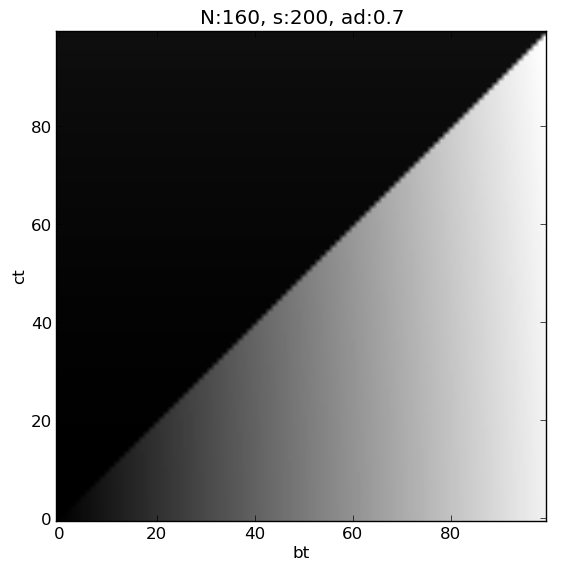
\includegraphics[width=0.5\textwidth]{expected_time_160_7.png}
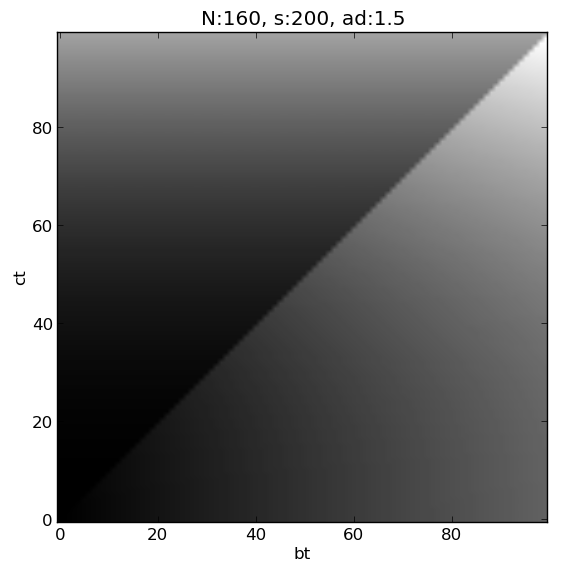
\includegraphics[width=0.5\textwidth]{expected_time_160_15.png}
\caption{Expected time for mating, dark is lower.}
\end{figure}
\end{frame}

\begin{frame}
\frametitle{An experiment, with ad=1, s=120}
\input{dessin_tikz_13_res.txt}
\end{frame}

\begin{frame}
\frametitle{An experiment, with ad=1, s=120}
\begin{figure}
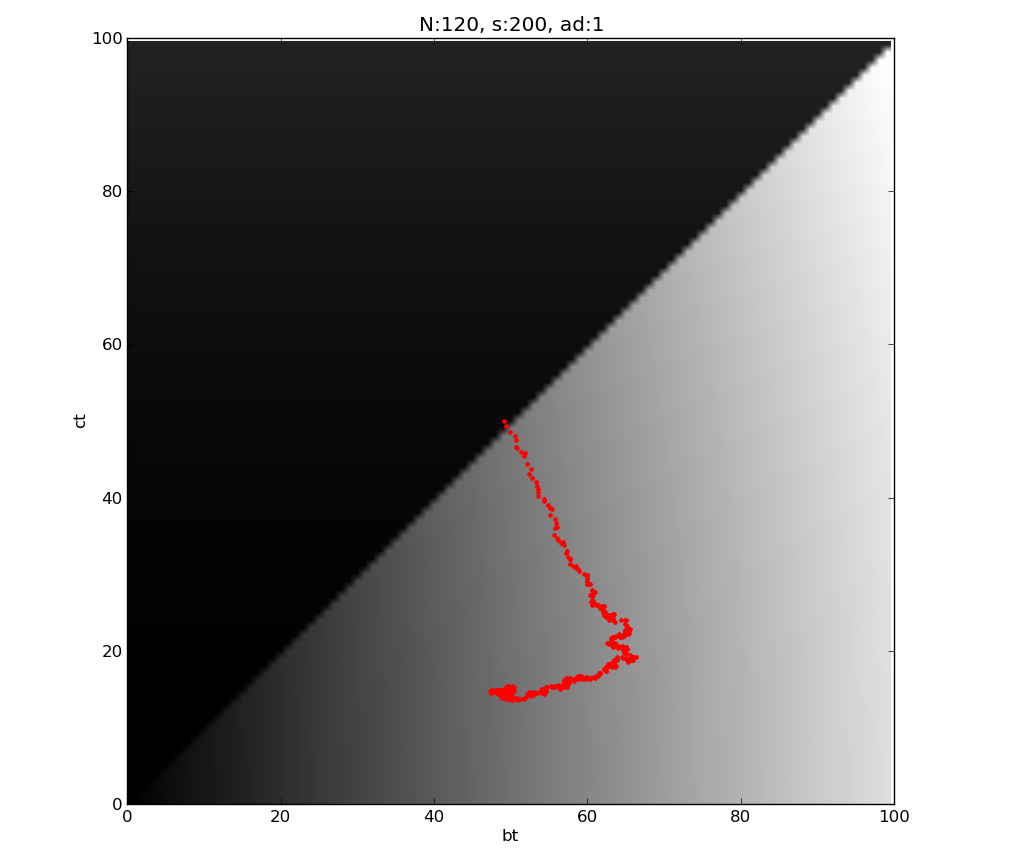
\includegraphics[width=0.5\textwidth]{120_1_traj.png}
\caption{Expected time for mating, dark is lower.}
\end{figure}
\end{frame}

\begin{frame}
\frametitle{With lower ad: 0.7}
\input{dessin_tikz_10_res.txt}
\end{frame}

\begin{frame}
\frametitle{With higher ad: 1.5}
\input{dessin_tikz_18_res.txt}
\end{frame}

\begin{frame}
\frametitle{With s=200}
\input{dessin_tikz_49_res.txt}
\end{frame}

\frame[containsverbatim]{
\frametitle{Questions?}
Thank you for your attention.
}



\end{document}
